\subsection{Equilibrium model}
\begin{frame}{Equilibrium model}
\label{sec:equilibrium_model}

\begin{columns}
\begin{column}{0.5\textwidth}

LLC works for TF\\
extend to KP with second node attribute

% The LLC model~(\autoref{sec:eberhardt}) attempts to describe causal effects from node value to another through unknown edges. The natural application to gene regulation would be to have each node represent both a gene and its protein product, node values $\boldsymbol{x}$ would represent gene expression levels, and edges would represent protein regulation. The node values can be absolute or relative protein concentrations, in our case log fold-change mRNA measurements~(\autoref{sec:yeast_data}).

% The direct causal effects from one protein to the expression of another makes sense when describing transcription factors that directly regulate gene expression, but is unsuitable when including protein kinases and other protein regulators, since their regulation are on another protein attribute that concentration, for instance the protein's level of phosphorylation. Their influence on the observed gene expression levels is only indirect, which would make them latent variables in LLC, where their effects will have to be described with $\boldsymbol{e}$ as linear effects.
% LLC can be extended to better model indirect regulation effect. Since many proteins can be assumed to be either transcription factors, kinases or phosphatases, it is possible to separate them in the model.

% In order to capture this indirectness, LLC is extended here by adding a second node attribute: "activity". Activity of a protein is meant to describe its state of phosphorylation but since it is unknown if a given protein is in its active form when phosphorylated or dephosphorylated, we generalize the concept of phosphorylation as protein activity.

% A graph in this model is therefore fully defined by a set of edges and nodes, where each edge are directed, so has source and target node attribute, has a signed edge value, and is either categorized as a transcription or activity regulating edge. Each node has three attributes: observed node value indicating relative concentration, unobserved activity attribute, and is category as either TF or PK. The "node value" refers to the observed node value if not explicitly referring to any of the three attributes. We use the simple assumption that a protein cannot be both a transcription regulator and an protein activity regulator, which means that edge types are implicitly known from the type of the edge source.

% The simplest case of regulation between node values is linear effects from node value to node value which can be described as by Eberhardt~et~al. The transcription factors will then have a linear regulation for directly observed node values, while the kinases have linear regulation on the activity attribute of nodes~(\autoref{eq:basic_eberhardt_extension}).


\begin{subequations}
\label{eq:basic_eberhardt_extension}
\begin{align}
x_i(t) &= \sum_{j \in \text{TF}} w_{ij} a_j(t-1) + e_i^{(x)}
\\
y_i(t) &= \sum_{j \in \text{KP}} w_{ij} a_j(t-1) + e_i^{(y)}
\\
\boldsymbol{x}(t) &= W I_\text{TF} \boldsymbol{a}(t-1) + \boldsymbol{e}_x
\\
\boldsymbol{y}(t) &= W I_\text{KP} \boldsymbol{a}(t-1) + \boldsymbol{e}_y
\end{align}
\end{subequations}
Node attributes:
\begin{conditions}
\boldsymbol{x}(t) & observed in data \\
\boldsymbol{y}(t) & hidden (KP regulated activity) \\
\boldsymbol{a}(t) & effective
\end{conditions}
% Here, $x_i(t)$ is the $i$-th directly observed node value, $y_i(t)$ the activity node attribute, each at discrete timestep $t$. $w_{ij}$ is the edge weight from protein $j$ to $i$, and $a_j(t-1)$ the effective amount of the $j$-th protein at time $t-1$. $e_i^{(x)}$ and $e_i^{(y)}$ are the error terms capturing latent, overlooked variables, and noise. The set $T$ and $P$ are the node indexes for transcription factors and protein kinases, so in matrix/vector notation we can combine all edges in a matrix $W$ where $I_T$ and $I_P$ are diagonal matrices where $I_T$ has 1s in the diagonal corresponding to indexes for TF nodes in $\boldsymbol{x}$, and similarly for $I_P$ in regard to PK node indexes. We sort the proteins with TFs first, followed by PKs~(\autoref{fig:W}).
% The matrix $W$ has zeros in its diagonal for the same reason as why this is enforced for $B$ in LLC~(\autoref{sec:eberhardt}).
\end{column}

\begin{column}{0.5\textwidth}
\begin{figure}[ht]
    \centering
    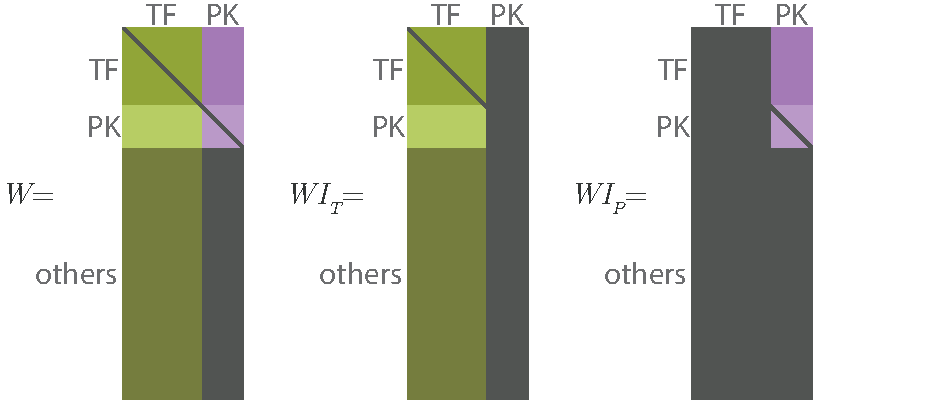
\includegraphics[width=\textwidth]{methods/fig/W.pdf}
    \caption{\textbf{\textit{W}.} Column = edge source, row = target. \\ \textcolor{darkgray}{Dark gray} = 0. Dimensions = $N \times (N_\text{TF} + N_\text{KP})$. }
    \label{fig:W}
\end{figure}
\end{column}
\end{columns}
\end{frame}

\begin{frame}{Equilibrium model}
% Since we are only observing~$\boldsymbol{x}$ we wish to have all other terms for hidden node values disappear which is possible since the model is linear~(\autoref{eq:first_equilibrium_final}).

% If we describe each of the terms as log fold-change versions of absolute measurements for knockout and wildtype experimental conditions, we can get the following~(\autoref{eq:second_equilibrium_def}).
$(t)$ omitted:
\begin{subequations}
\label{eq:second_equilibrium_def}
\begin{equation}
a_i^{(\text{ko})} = y_i^{(\text{ko})} \cdot x_i^{(\text{ko})}
\quad,\quad
a_i^{(\text{wt})} = y_i^{(\text{wt})} \cdot x_i^{(\text{wt})}
\end{equation}\begin{equation}
x_i = \log \frac{x_i^{(\text{ko})}}{x_i^{(\text{wt})}}
\quad,\quad
y_i = \log \frac{y_i^{(\text{ko})}}{y_i^{(\text{wt})}}
\quad,\quad
a_i = \log \frac{a_i^{(\text{ko})}}{a_i^{(\text{wt})}}
= \log \frac{y_i^{(\text{ko})} x_i^{(\text{ko})}}{y_i^{(\text{wt})} x_i^{(\text{wt})}}
= y_i + x_i    
\end{equation}\begin{equation}
\boldsymbol{a}(t) = \boldsymbol{y}(t) + \boldsymbol{x}(t)
\end{equation}
\end{subequations}

% Here $y_i^{(\text{ko})}$ and $y_i^{(\text{wt})}$ are absolute node values, which are typically unmeasured, describing the effective fraction of each protein.

% Owing to the simplicity of a linear model we can cancel out hidden node values as before~(\autoref{eq:second_equilibrium_final}).
Can be shown to converge for $t\rightarrow\infty$
\begin{subequations}
\label{eq:second_equilibrium_final}
\begin{align}
\boldsymbol{a} &= 
    \left(WI_\text{KP}\boldsymbol{a} + \boldsymbol{e}_y\right) + \boldsymbol{x}
\\
\left(I-WI_\text{KP}\right) \boldsymbol{a} &=
    \boldsymbol{e}_y + \boldsymbol{x}
\\
\boldsymbol{a} &=
    \left(I-WI_\text{KP}\right)^{-1} \left(\boldsymbol{e}_y + \boldsymbol{x}\right)
\\
\boldsymbol{x} &=
    WI_\text{TF} \left(I-WI_\text{KP}\right)^{-1} \left(\boldsymbol{e}_y + \boldsymbol{x}\right) + \boldsymbol{e}_x
\\
&= WI_\text{TF} \left(I-WI_\text{KP}\right)^{-1} \boldsymbol{x} + \boldsymbol{e}
\\
\label{eq:second_equilibrium_final.f}
&= B\boldsymbol{x} + \boldsymbol{e}
\enspace,\enspace B = WI_\text{TF} \left(I-WI_\text{KP}\right)^{-1}
\end{align}
\end{subequations}


% Again, the resulting description of observed node values $\boldsymbol{x}$ at equilibrium as a function of itself, can be written as by Eberhardt~et~al. with an extension to $B$. The extension of $B$ is identical to the one at \autoref{eq:first_equilibrium_final.e} with the exception of the 2.
% This model was chosen as the main method going forward based on better intuition in its design, as well as through tests showing little performance difference. 
\end{frame}


\begin{frame}{Equilibrium model - simulation}
\label{sec:prim}

Initial conditions (fig.~\ref{fig:KO_RNA_hist}):
\begin{subequations}
\begin{align}
\boldsymbol{x}_{\mathcal{U}_k} &= 0
\\
\boldsymbol{x}_{\mathcal{J}_k} &\sim \mathcal{N}(\mu=-4, \sigma=1)
\end{align}
\end{subequations}

Simple iteration of eq. \ref{eq:second_equilibrium_final.f} \\
% , where the parameters are chosen based on the observations in . $\boldsymbol{x}(t)$ is then calculated iteratively with \autoref{eq:second_equilibrium_final.f} until approximate convergence is reached, otherwise it will be stopped after 10,000 iterations. Approximate convergence is reached when it holds
Approx. convergence:
\begin{equation}
\label{eq:convergence}
\tfrac{1}{N} \sum_{i=1}^N |x_i(t)-x_i(t-1)| < \epsilon_{tol} \,,\,\epsilon_{tol}=10^{-7}
\end{equation}

\end{frame}

\begin{frame}{Equlibrium model - inference}
\label{sec:equilibrium_inference}

% The obvious way to implement the equations described in \autoref{eq:second_equilibrium_final} in order to infer graph edges will be by applying the algorithm of Eberhardt~et~al., which gives us $B$, and with \autoref{eq:second_equilibrium_final.f} solve for $W$. This cannot be done analytically but is implemented as a gradient descent method where the difference between $B$ and the right hand side of its definition in \autoref{eq:second_equilibrium_final.f} is minimized~(\autoref{eq:loss_B}).
% This approach is referred to as the $B$-method. If there is no covariance matrices for $\boldsymbol{x}_k$ available, $T_{\boldsymbol{x}_k}$ will have to be found using \autoref{eq:t_regress}, which only describes single intervention experiments.

Minimizing a loss function

% Another approach that allows for the inclusion of multiple interventions in an experiment is to minimize~$\boldsymbol{e}$ which is also an attempt at having the least amount of latent variables in the system.
% This approach is referred to as the $\boldsymbol{e}$-minimization method.
% It works by describing the systems of equations from the model in a symbolic math or neural network library in Python. The libraries help by constructing functions for gradients $\dv{\mathcal{L}}{w_{ij}}$, where $\mathcal{L}$ is the loss function and $w_{ij}$ a parameter in $W$. We then minimize the gradient using Adam gradient descent until perceived convergence~\cite{adam}.
% The graph will be sparse which is enforced through L1-regularization. The loss minimized for the $\boldsymbol{e}$-method and $B$-method are:

\begin{subequations}
\label{eq:loss}
\begin{align}
\mathcal{L}_B &=
\sum_{j=1}^N \sum_{i=1}^N
\left(b_{ij} - b_{ij}^{(\text{LLC})}\right)^2
+ \lambda_T \sum_{j \in \text{TF}} \sum_{i=1}^N |w_{ij}| + \lambda_\text{KP} \sum_{j \in \text{KP}} \sum_{i=1}^{N_\text{TF} + N_\text{KP}} |w_{ij}|
\label{eq:loss_B}
\\
\mathcal{L}_{\boldsymbol{e}} &=
\sum_{i=1}^N e_i^2 + \lambda_\text{TF} \sum_{j \in \text{TF}} \sum_{i=1}^N |w_{ij}| + \lambda_\text{KP} \sum_{j \in \text{KP}} \sum_{i=1}^{N_\text{TF} + N_\text{KP}} |w_{ij}|
\label{eq:loss_e}
\end{align}
\end{subequations}

% Here, $\lambda_T$ and $\lambda_P$ are regularization hyperparameters for $W I_T$ and $W I_P$, which means they are chosen to achieve a desired level of sparsity in each of those parts of the weight matrix $W$. They are not necessarily chosen as two different values. $b_{ij}^{(\text{LLC})}$ are values of $B_{\text{LLC}}$ found using LLC. $b_{ij}$ are elements of $B$ which is a function of the trainable parameters in $W$ as described in~\autoref{eq:second_equilibrium_final.f}.


\end{frame}





